\documentclass[tikz]{standalone}
\usepackage{pgfplots}
\pgfplotsset{width=14cm, height=9cm, compat=1.18}
\usepackage{tikz}
\usetikzlibrary{spy}
\usepackage{gensymb}
\usepackage{amsmath}
\usepackage[export]{adjustbox} % brings valign

% Dirtily adapted from: https://tex.stackexchange.com/questions/42342/how-to-change-the-line-width-of-the-lines-connecting-spies-and-the-spied-region
% (dirty because I set some line parameters both in the tikzset AND in its invokation)
\begin{document}
	\tikzset{
		my spy on/.style={#1},
		my spy/.style={
			spy scope={
				every spy on node/.style={
					draw,
					circle,
					densely dashed, 
					size=2.5cm,
					my spy on,
				},
				every spy in node/.style={
					draw,
					red,
					densely dashed,
					size=2.5cm,
					very thick,
					circle,
				},
				#1
			}
		}
	}
	%spy using outlines={circle, very thick, dashed, magnification=6, size=2.5cm, connect spies}
	\begin{tikzpicture}[my spy, magnification=6]
		\node[inner sep=0pt, anchor=west] (strips) at (0,0) {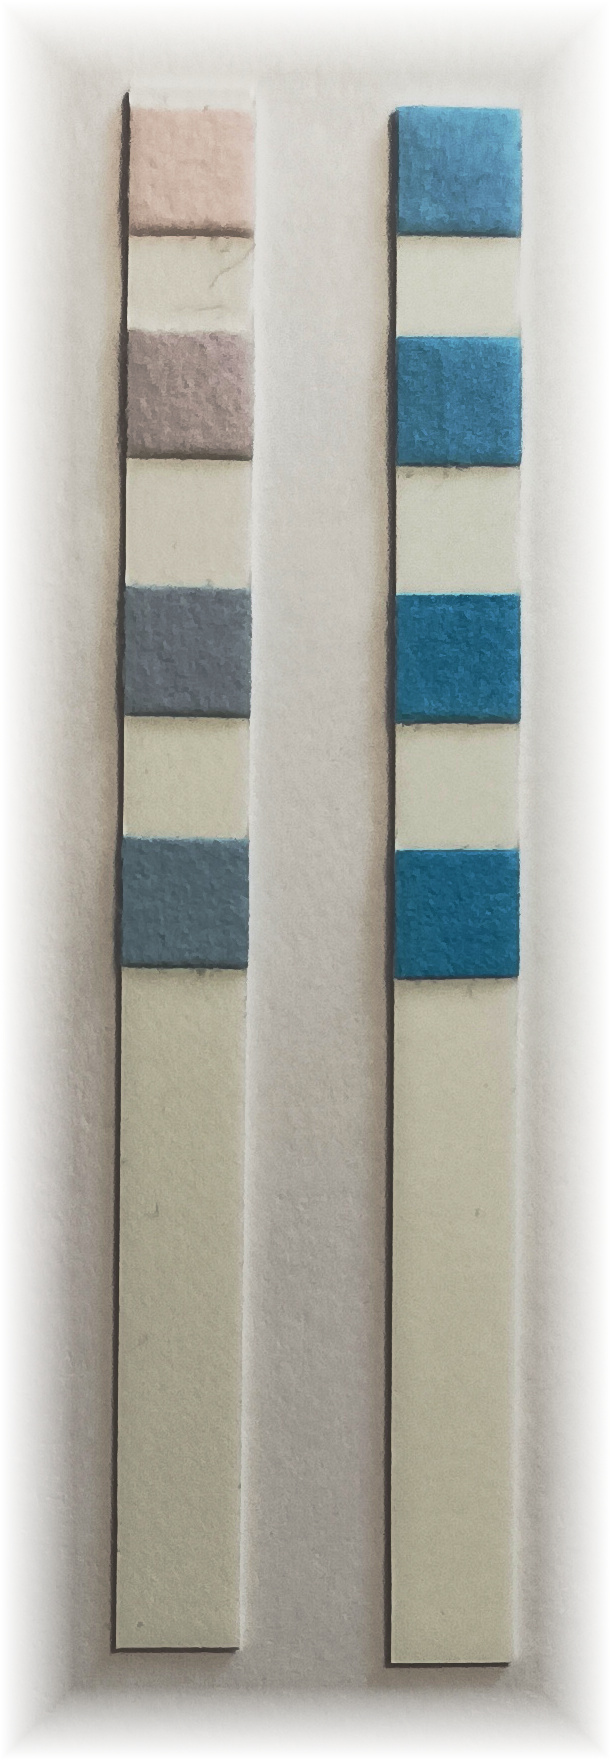
\includegraphics[height=7cm]{../strips}};
		\node[inner sep=0pt, anchor=east] (patcharm) at (14,0) {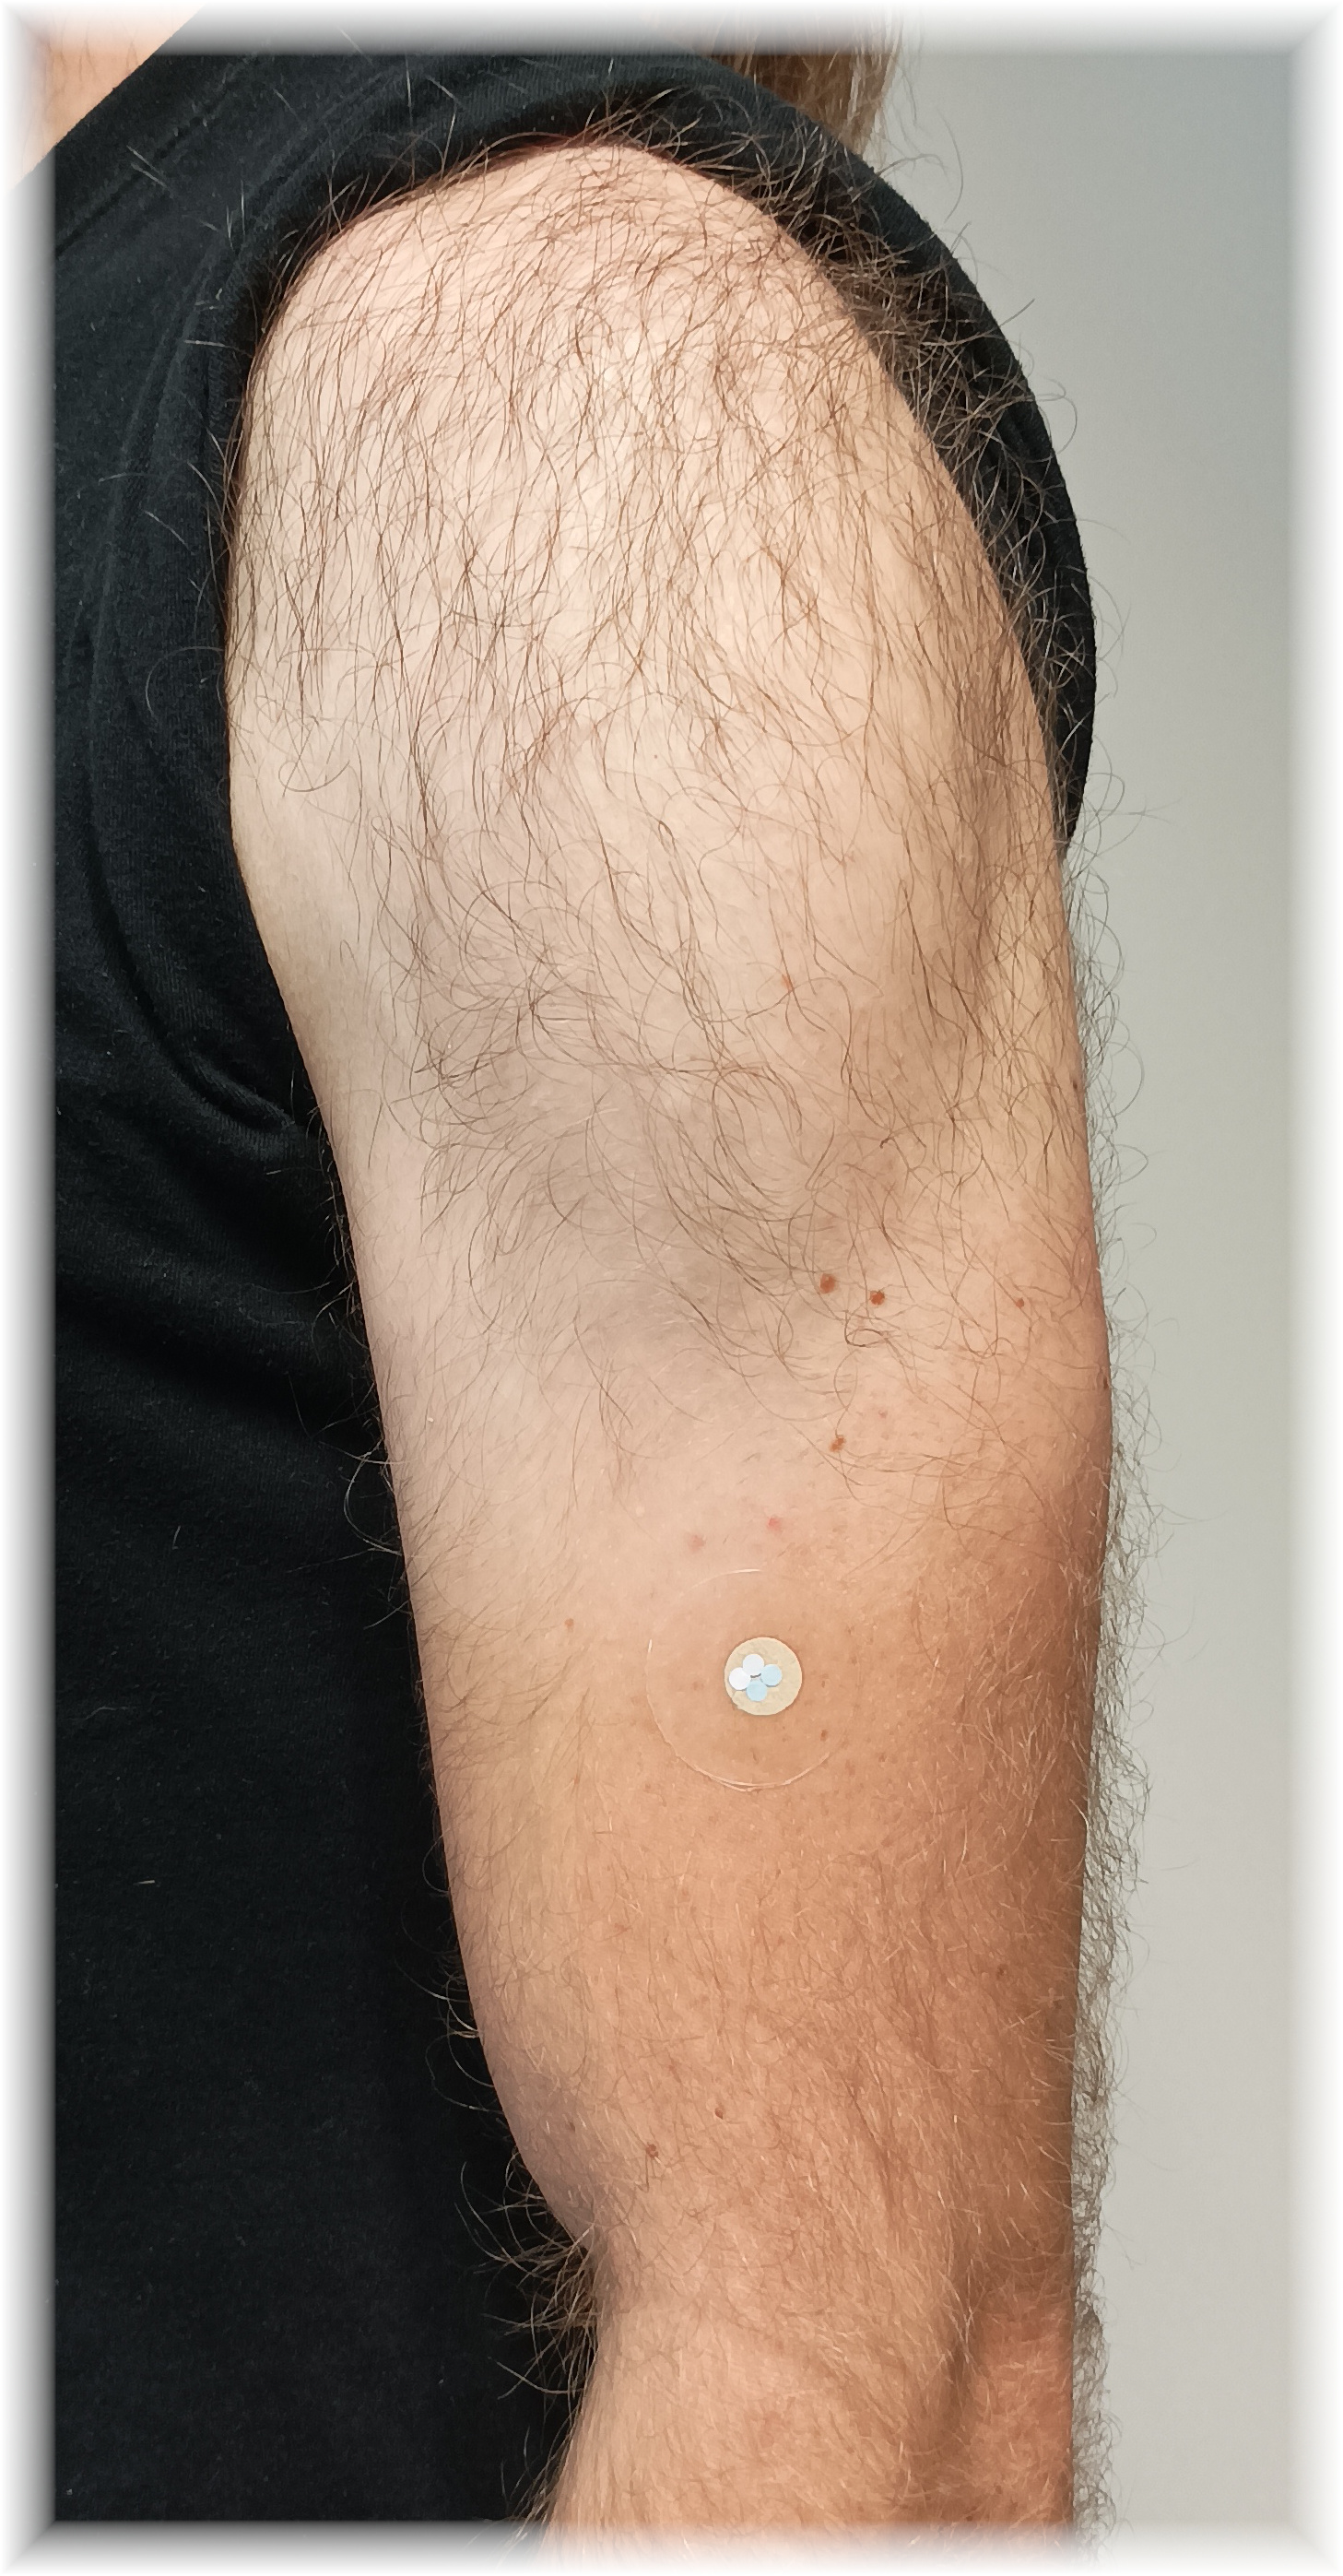
\includegraphics[height=7cm]{../patch_arm}};
		\spy [red, very thick, spy connection path={\draw[red, very thick, densely dashed] (tikzspyonnode) -- (tikzspyinnode);}, my spy on={red, very thick}] on (12.42,-1.06)
		in node [left] at (11.25,-2.);
		\path (strips) -- (patcharm) node[midway] (b) {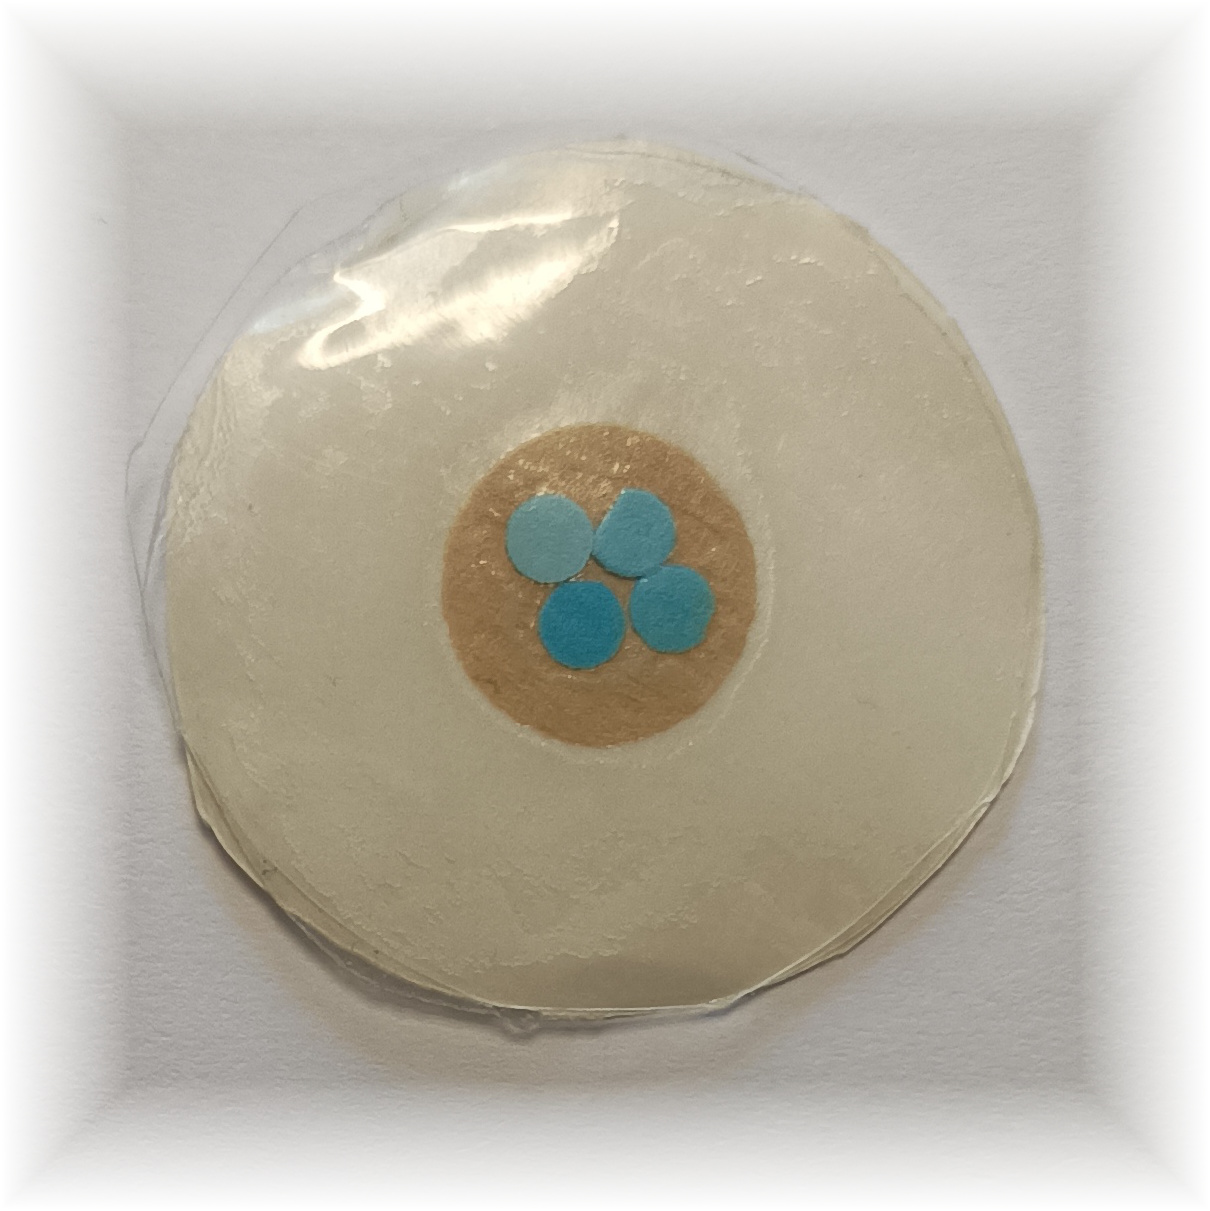
\includegraphics[height=7cm]{../patch_full}};
	\end{tikzpicture}
\end{document}